%页面设置
\documentclass[a4paper]{article}
\usepackage[top=1in,bottom=1in,left=1in,right=1in]{geometry}
%\usepackage[utf8]{inputenc}
\usepackage{titlesec} %标题位置,有center,raggedleft,raggedright三个选项
\linespread{1.3}\selectfont
%本地化
\usepackage{fontspec}
\setmainfont{SimSun}
\XeTeXlinebreaklocale "zh"
\XeTeXlinebreakskip = 0pt plus 1pt minus 0.1pt
%数学
\usepackage{amsmath}
\makeatletter
\def\verbatim@font{} %如果使用roman字体族,将sffamily改成rmfamily
\makeatother
%文档
\begin{document}
\title{现代控制理论}
\author{闫鹏}
\date{}
\maketitle
\noindent
\section*{第一题}
\mbox{已知 }$ A=\left(\begin{array}{ccc} 1 & 0 & -1\\ 0 & -2 & 0\\ -1 & 0 & 2 \end{array}\right) $,
$ B=\left(\begin{array}{c} 0\\ 0\\ 1 \end{array}\right) $,  $ C=\left(\begin{array}{ccc} 1 & 0 & 0 \end{array}\right)$. \\
$ G(s)=C(sI-A)^{-1}B $,\mbox{且}
$ (sI-A)=\left(\begin{array}{ccc} s - 1 & 0 & 1\\ 0 & s + 2 & 0\\ 1 & 0 & s - 2 \end{array}\right) $ \\
\mbox{通过初等函数法求逆矩阵} \\
\begin{displaymath}
\left(\begin{array}{cccccc} s - 1 & 0 & 1 & 1 & 0 & 0\\ 0 & s + 2 & 0 & 0 & 1 & 0\\ 1 & 0 & s - 2 & 0 & 0 & 1 \end{array}\right) = \left(\begin{array}{cccccc} 1 & 0 & 0 & \frac{s - 2}{s^2 - 3\, s + 1} & 0 & -\frac{1}{s^2 - 3\, s + 1}\\ 0 & 1 & 0 & 0 & \frac{1}{s + 2} & 0\\ 0 & 0 & 1 & -\frac{1}{s^2 - 3\, s + 1} & 0 & \frac{s - 1}{s^2 - 3\, s + 1} \end{array}\right)
\end{displaymath} \\
\mbox{故逆矩阵 }$(sI-A)^{-1}= \left(\begin{array}{ccc} \frac{s - 2}{s^2 - 3\, s + 1} & 0 & -\frac{1}{s^2 - 3\, s + 1}\\ 0 & \frac{1}{s + 2} & 0\\ -\frac{1}{s^2 - 3\, s + 1} & 0 & \frac{s - 1}{s^2 - 3\, s + 1} \end{array}\right) $ \\
$$ G(s)=C(sI-A)^{-1}B = \left(\begin{array}{ccc} 1 & 0 & 0 \end{array}\right) \left(\begin{array}{ccc} \frac{s - 2}{s^2 - 3\, s + 1} & 0 & -\frac{1}{s^2 - 3\, s + 1}\\ 0 & \frac{1}{s + 2} & 0\\ -\frac{1}{s^2 - 3\, s + 1} & 0 & \frac{s - 1}{s^2 - 3\, s + 1} \end{array}\right) \left(\begin{array}{c} 0\\ 0\\ 1 \end{array}\right) =   \frac{s + 2}{ - s^3 + s^2 + 5\, s - 2} $$ \\
\mbox{上下通分可得 }$G(s)= \frac{s + 2}{ - s^3 + s^2 + 5\, s - 2} $
\begin{verbatim}[matlab]
[num ,den]=ss2tf(A,B,C,D)
num =
     0     0    -1    -2
den =
     1    -1    -5     2
\end{verbatim} 
\section*{第二题} 
状态转移矩阵
\begin{equation*} 
\begin{split}
\Phi(t) &= e^{A}t=\mathcal{L}^{-1}[(sI-A)^{-1}]=\mathcal{L}^{-1} \left(\begin{array}{ccc} \frac{s - 2}{s^2 - 3\, s + 1} & 0 & -\frac{1}{s^2 - 3\, s + 1}\\ 0 & \frac{1}{s + 2} & 0\\ -\frac{1}{s^2 - 3\, s + 1} & 0 & \frac{s - 1}{s^2 - 3\, s + 1} \end{array}\right) \\
&= \left(\begin{array}{ccc} \mathrm{e}^{\frac{3\, t}{2}}\, \left(\cosh\!\left(\frac{\sqrt{5}\, t}{2}\right) - \frac{\sqrt{5}\, \sinh\!\left(\frac{\sqrt{5}\, t}{2}\right)}{5}\right) & 0 & -\frac{2\, \sqrt{5}\, \mathrm{e}^{\frac{3\, t}{2}}\, \sinh\!\left(\frac{\sqrt{5}\, t}{2}\right)}{5}\\ 0 & \mathrm{e}^{- 2\, t} & 0\\ -\frac{2\, \sqrt{5}\, \mathrm{e}^{\frac{3\, t}{2}}\, \sinh\!\left(\frac{\sqrt{5}\, t}{2}\right)}{5} & 0 & \mathrm{e}^{\frac{3\, t}{2}}\, \left(\cosh\!\left(\frac{\sqrt{5}\, t}{2}\right) + \frac{\sqrt{5}\, \sinh\!\left(\frac{\sqrt{5}\, t}{2}\right)}{5}\right) \end{array}\right)
\end{split}
\end{equation*}
\mbox{已知 }x(t)=$\Phi(t)x(0)+\int^{t}_{0}(t-\tau)Bu(\tau)d\tau$,$x(0)= \left(\begin{array}{c} 1\\ 2\\ 1 \end{array}\right)$

\begin{align*}
\Phi(t)x(0) & = 
\left(\begin{array}{c} \mathrm{e}^{\frac{3\, t}{2}}\, \left(\cosh\!\left(\frac{\sqrt{5}\, t}{2}\right) - \frac{\sqrt{5}\, \sinh\!\left(\frac{\sqrt{5}\, t}{2}\right)}{5}\right) - \frac{2\, \sqrt{5}\, \mathrm{e}^{\frac{3\, t}{2}}\, \sinh\!\left(\frac{\sqrt{5}\, t}{2}\right)}{5} \\ 2\, \mathrm{e}^{- 2\, t}\\ \mathrm{e}^{\frac{3\, t}{2}}\, \left(\cosh\!\left(\frac{\sqrt{5}\, t}{2}\right) + \frac{\sqrt{5}\, \sinh\!\left(\frac{\sqrt{5}\, t}{2}\right)}{5}\right) - \frac{2\, \sqrt{5}\, \mathrm{e}^{\frac{3\, t}{2}}\, \sinh\!\left(\frac{\sqrt{5}\, t}{2}\right)}{5} \end{array}\right) \\
\int^{t}_{0}\Phi(t-\tau)Bu(\tau)d\tau & = 
\end{align*}

\mbox{故 }$ x(t)=\\
\left(\begin{array}{c} \frac{\mathrm{e}^{\frac{3\, t}{2} - \frac{\sqrt{5}\, t}{2}}}{2} + \frac{\mathrm{e}^{\frac{3\, t}{2} + \frac{\sqrt{5}\, t}{2}}}{2} + \frac{3\, \sqrt{5}\, \mathrm{e}^{\frac{3\, t}{2} - \frac{\sqrt{5}\, t}{2}}}{10} - \frac{3\, \sqrt{5}\, \mathrm{e}^{\frac{3\, t}{2} + \frac{\sqrt{5}\, t}{2}}}{10} + \frac{\sqrt{5}\, \left(\mathrm{e}^{\frac{3\, t}{2} - \frac{\sqrt{5}\, t}{2}} - 1\right)\, \left(\sqrt{5} + 3\right)}{10} + \frac{\sqrt{5}\, \left(\mathrm{e}^{\frac{3\, t}{2} + \frac{\sqrt{5}\, t}{2}} - 1\right)\, \left(\sqrt{5} - 3\right)}{10}\\ 2\, \mathrm{e}^{- 2\, t}\\ \mathrm{e}^{\frac{3\, t}{2} - \frac{\sqrt{5}\, t}{2}} + \mathrm{e}^{\frac{3\, t}{2} + \frac{\sqrt{5}\, t}{2}} + \frac{\sqrt{5}\, \mathrm{e}^{\frac{3\, t}{2} - \frac{\sqrt{5}\, t}{2}}}{5} - \frac{\sqrt{5}\, \mathrm{e}^{\frac{3\, t}{2} + \frac{\sqrt{5}\, t}{2}}}{5} - 1 \end{array}\right) $ \\

\begin{verbatim}[matlab]
syms t,tao %定义时间变量t, tao为符号
A=[1 0 -1; 0 -2 0; -1 0 2]; B=[0; 0; 1]; x0=[1; 2; 1] %输入系统状态方程和初始值
xt=expm(A*t)*x0+int(expm(A*(t-tao))*B*1,tao,0,t) %求非齐次解
绘出单位阶跃响应的系统状态轨迹图
t=0:0.1:10
plot(t, exp((3*t)/2 - (5^(1/2)*t)/2)/2 + exp((3*t)/2 + (5^(1/2)*t)/2)/2 + (3*5^(1/2)*exp((3*t)/2 - (5^(1/2)*t)/2))/10 - (3*5^(1/2)*exp((3*t)/2 + (5^(1/2)*t)/2))/10 + (5^(1/2)*(exp((3*t)/2 - (5^(1/2)*t)/2) - 1)*(5^(1/2) + 3))/10 + (5^(1/2)*(exp((3*t)/2 + (5^(1/2)*t)/2) - 1)*(5^(1/2) - 3))/10,t,  2*exp(-2*t), t, exp((3*t)/2 - (5^(1/2)*t)/2) + exp((3*t)/2 + (5^(1/2)*t)/2) + (5^(1/2)*exp((3*t)/2 - (5^(1/2)*t)/2))/5 - (5^(1/2)*exp((3*t)/2 + (5^(1/2)*t)/2))/5 - 1)
\end{verbatim}
\begin{figure}[h]  %控制单张图片位置h
\centering
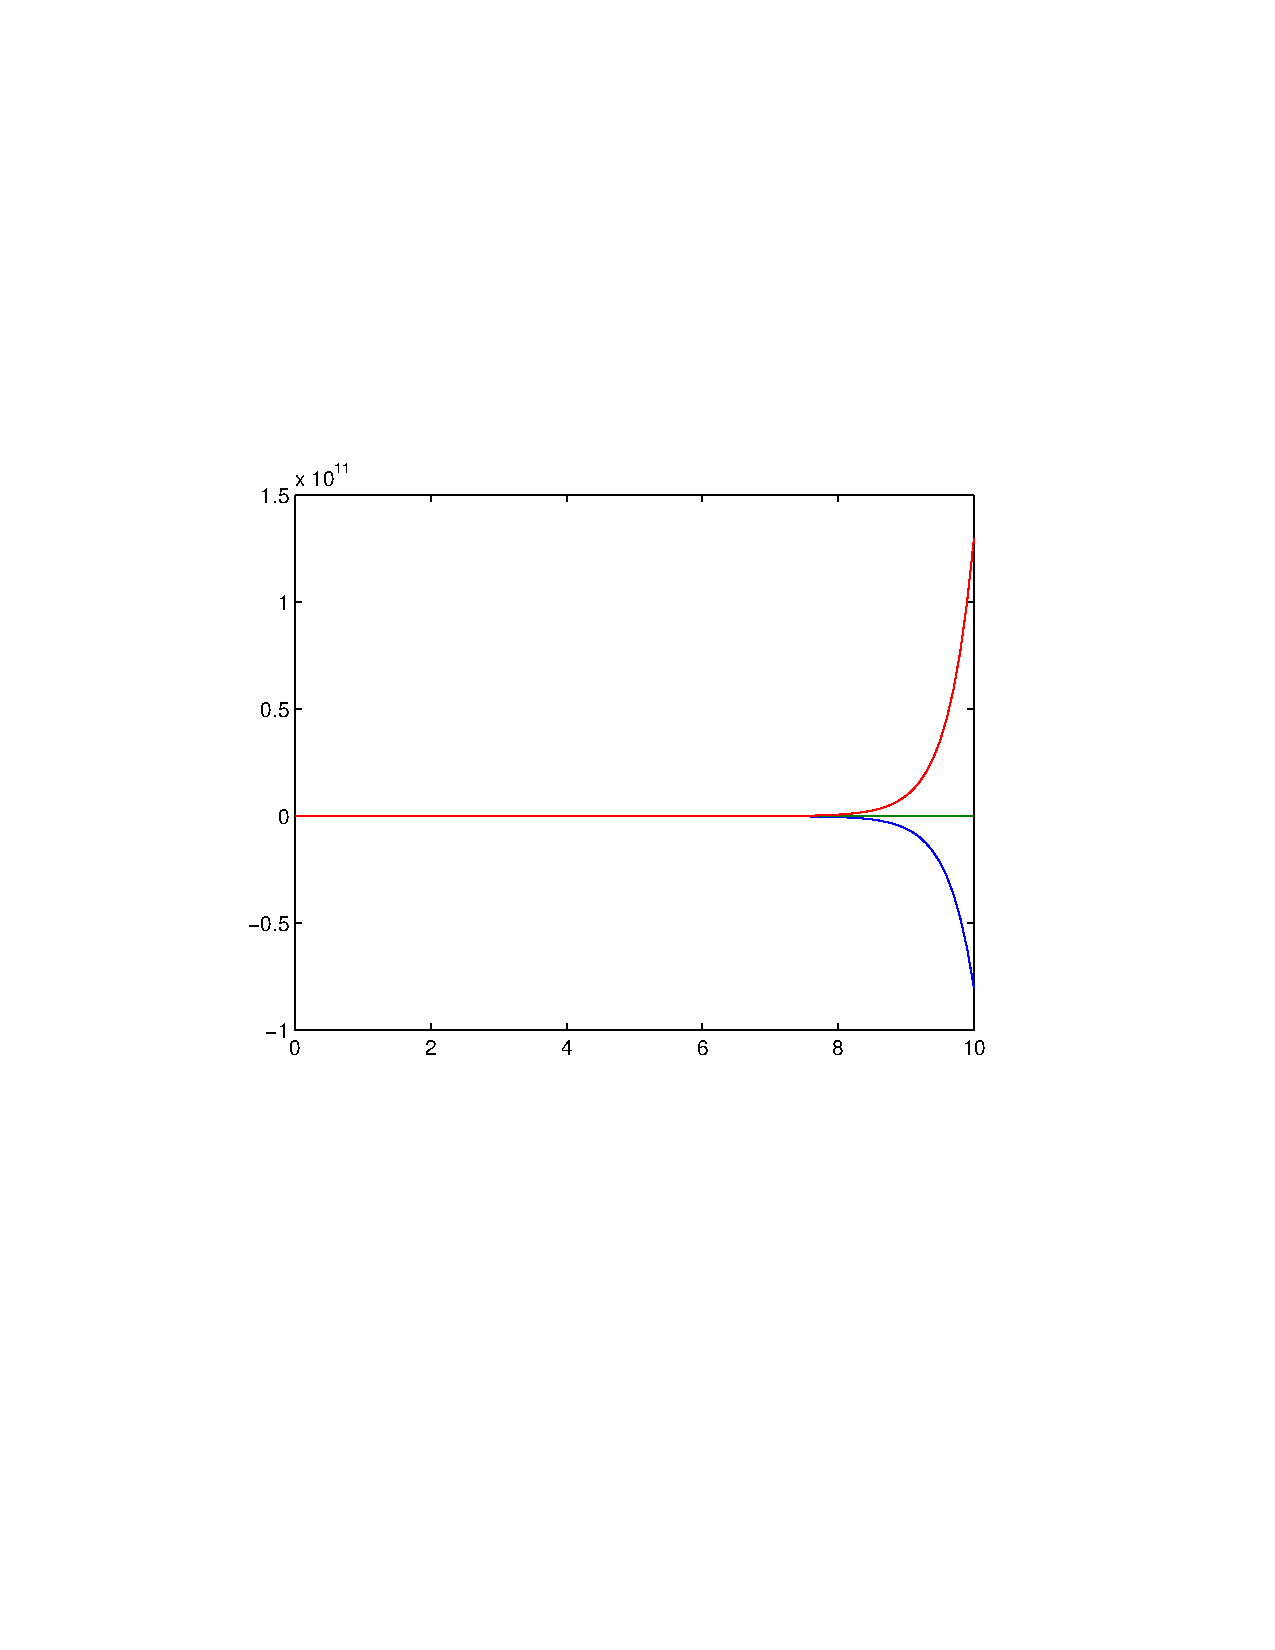
\includegraphics{num2} 
\caption{单位阶跃响应的系统状态轨迹图}
\end{figure}

\section*{第三题}
状态方程的能空检验矩阵$Qc=\left(\begin{array}{ccc} B & AB & A^{2}B \end{array}\right)$ \\
$A= \left(\begin{array}{ccc} 1 & 0 & -1\\ 0 & -2 & 0\\ -1 & 0 & 2 \end{array}\right) $,
$AB=  \left(\begin{array}{c} -1\\ 0\\ 2 \end{array}\right) $,
$A^{2}B=  \left(\begin{array}{c} -3\\ 0\\ 5 \end{array}\right) $ \\
\mbox{所以 }$Qc= \left(\begin{array}{ccc} 0 & -1 & -3\\ 0 & 0 & 0\\ 1 & 2 & 5 \end{array}\right) $
\\可知该矩阵的佚为2,小于3,所以状态不完全能控\\
\noindent\\
状态方程的能观矩阵$Qo=\left(\begin{array}{ccc} C & CA & CA^{2} \end{array}\right) $
\\ $C= \left(\begin{array}{ccc} 1 & 0 & 0 \end{array}\right)$, 
$CA=\left(\begin{array}{ccc} 1 & 0 & -1 \end{array}\right)$,
$CA^{2}=\left(\begin{array}{ccc} 2 & 0 & -3 \end{array}\right)$ \\
\mbox{所以 }$Qo=\left(\begin{array}{ccc} 1 & 0 & 0\\ 1 & 0 & -1\\ 2 & 0 & -3 \end{array}\right)$
\\可知该矩阵的佚为2,小于3,所以状态不完全能观

\begin{verbatim}[matlab]
A=[1 0 -1; 0 -2 0; -1 0 2]; B=[0; 0; 1]; %输入系统状态方程
Qc=ctrb(A,B) %求系统能控性矩阵
rank(Qc) %求系统能控性矩阵的佚
ans = 2 %能控性矩阵的佚为2,所以系统不能控
 
A=[1 0 -1; 0 -2 0; -1 0 2]; C=[1 0 0] %输入系统状态方程;   
Qo=obsv(A,C)  %求系统能观性矩阵
rank(Qo) %求系统能控性矩阵的佚
ans = 2 %能观性矩阵的佚为2,所以系统不能观
\end{verbatim}
\section*{第四题}
欲使连续系统稳定,必须使特征方程 $|sI-A|=0$ 的根,亦即矩阵A的特征值,全部位于s平面的左半开平面上。
\\系统矩阵A为非奇异线性定常系统,$x_{e}=0$即原点,是系统的唯一平衡状态,其稳定性可由劳斯判据得到。
\\已知$|sI-A|=s^3 - s^2 - 5\, s + 2 =0 $
\\列出劳斯表可得
\begin{table*}[!h]
\centering
\caption{劳斯表}
\begin{tabular}{c  c  c}  
$s^{3}$ & 1 & -5 \\ 
$s^{2}$ & -1 & 2 \\ 
$s^{1}$ & -3 & \\ 
$s^{0}$ & 2 & 
\end{tabular}
\end{table*}
\noindent
由劳斯稳定判据可知,系统有两个正实根,即在该平衡点不稳定。

\begin{verbatim}[matlab] 
det(s*eye(3)-A) = s^3 - s^2 - 5*s + 2 %求特征方程
solve(s^3 - s^2 - 5*s + 2) %求特征方程解 
ans =
              -2
 5^(1/2)/2 + 3/2=2.618
 3/2 - 5^(1/2)/2=0.382
可知系统有两个解在s平面的右半开平面上,该平衡点不稳定
\end{verbatim}

\section*{第五题}
\emph{能控性分解}\\
如上已知系统能控矩阵秩为2,小于3,故系统不完全能控。\\
$Qc= \left(\begin{array}{ccc} 0 & -1 & -3\\ 0 & 0 & 0\\ 1 & 2 & 5 \end{array}\right) $ \\
\mbox{取Qc中线性独立的两列向量,这里取第一、二列,再补充一个与其他列向量无关的列向量 }$\left(\begin{array}{c} 0\\ 1\\ 0 \end{array}\right)$ \\
\mbox{可得到 }$Pc^{-1}=\left(\begin{array}{ccc} 0 & -1 & 0\\ 0 & 0 & 1\\ 1 & 2 & 0 \end{array}\right)$,$Pc=\left(\begin{array}{ccc} 2 & 0 & 1\\ -1 & 0 & 0\\ 0 & 1 & 0 \end{array}\right)$ \\
\mbox{则 }$ \bar{A} =P_{c}AP_{c}^{-1}= \left(\begin{array}{ccc} 0 & -1 & 0\\ 1 & 3 & 0\\ 0 & 0 & -2 \end{array}\right)$,
$ \bar{B} =P_{c}B=\left(\begin{array}{c} 1\\ 0\\ 0 \end{array}\right)$,
$ \bar{C} =CP_{c}=\left(\begin{array}{ccc} 0 & -1 & 0 \end{array}\right)$
\noindent \\
能控子系统方程为
\begin{align*}
\dot{\bar{x}}_{c} &=  \left(\begin{array}{cc} 0 & -1\\ 0 & 0 \end{array}\right)x_{c}+\left(\begin{array}{c} 1\\ 0 \end{array}\right)u \\ 
y_{1} &= \left(\begin{array}{cc} 0 & -1 \end{array}\right)\bar{x}_{c}
\end{align*}
不能控子系统动态方程为
\begin{align*}
\dot{\bar{x}}_{\bar{c}} &= -2\bar{x}_{\bar{c}} \\
y_{2} &= 0
\end{align*}
\emph{能观性分解}\\
如上已知系统能观矩阵秩为2,小于3,故系统不完全能观。\\
$$ Q_{o}= \left(\begin{array}{ccc} 1 & 0 & 0\\ 1 & 0 & -1\\ 2 & 0 & -3 \end{array}\right)$$ \\
取$Q_{o}$中线性独立的两行向量,这里取第一、二行,再补充一个与其他行向量无关的行向量 $\left(\begin{array}{ccc} 0 & 1 & 0 \end{array}\right)$ \\
可得到$ P_{o}= \left(\begin{array}{ccc} 1 & 0 & 0\\ 1 & 0 & -1\\ 0 & 1 & 0 \end{array}\right), P_{o}^{-1}=\left(\begin{array}{ccc} 1 & 0 & 0\\ 0 & 0 & 1\\ 1 & -1 & 0 \end{array}\right)$ \\
则$ \bar{A}=P_{o}AP_{o}^{-1}= \left(\begin{array}{ccc} 0 & 1 & 0\\ -1 & 3 & 0\\ 0 & 0 & -2 \end{array}\right),
\bar{B}=P_{o}B= \left(\begin{array}{c} 0\\ -1\\ 0 \end{array}\right),
\bar{C}=CP_{o}^{-1}= \left(\begin{array}{ccc} 1 & 0 & 0 \end{array}\right)$ \\
能观子系统方程为\\
\begin{align*}
\bar{x}_{o} &= \left(\begin{array}{cc} 0 & 1\\ -1 & 3 \end{array}\right)\bar{x}_{o}+\left(\begin{array}{c} 0\\ -1 \end{array}\right)u \\
y_1 &= \left(\begin{array}{cc} 1 & 0 \end{array}\right)\bar{x}_o
\end{align*}
不能观子系统方程为\\
\begin{align*}
\dot{\bar{x}}_{\bar{o}} &= -2\bar{x}_o \\
y_2 &= 0
\end{align*}
%验证
\begin{verbatim}[matlab]
能控性分解
A=[1 0 -1; 0 -2 0; -1 0 2]; B=[0; 0; 1]; C=[1 0 0];  %输入系统状态方程
Qc=ctrb(A,B) %求系统能控性矩阵
rank(Qc) = 2 %求系统能控性矩阵的佚  
能控性矩阵的佚为2,所以系统不完全能控,可以按能控性分解
[Ac, Bc, Cc, T, K]=ctrbf(A, B,C)
Ac =
    -2     0     0
     0     1     1
     0     1     2
Bc =
     0
     0
     1
Cc =
     0    -1     0
T =
     0     1     0
    -1     0     0
     0     0     1
K =
     1     1     0

能观性分解
Qo=obsv(A,C)  %求系统能观性矩阵   
rank(Qo) = 2 %求系统能控性矩阵的佚
能观性矩阵的佚为2,所以系统不完全能观,可以按能观性分解
[Ao, Bo, Co, T, K]=obsvf(A, B,C)
Ao =
    -2     0     0
     0     2     1
     0     1     1
Bo =
     0
    -1
     0
Co =
     0     0     1
T =
     0     1     0
     0     0    -1
     1     0     0
K =
     1     1     0     
\end{verbatim}
\section*{第六题}
已知$A=\left(\begin{array}{ccc} 1 & 0 & -1\\ 0 & -2 & 0\\ -1 & 0 & 2 \end{array}\right)$, 通过初等函数法可求A的特征值为$ -2, 0.382, 2.618$ \\
系统有两个特征值为正,故系统不稳定。同时由定理3-2可知,系统不能控。不能控子系统特征值为-2,符合可镇定条件。 \\
\mbox{故原系统可用状态反馈实现镇定,镇定后的极点设为 }$ -1 \pm j $。 \\
\mbox{能控子系统方程为 }$Xc.=AcXc+Bcu= \left(\begin{array}{cc} 0 & -1\\ 1 & 3 \end{array}\right)Xc+\left(\begin{array}{cc} 1 & 0 \end{array}\right)u$ \\
\mbox{引入状态反馈 }$u=V-K_cx_c$,设$ K_c=\left(\begin{array}{cc} k_1 & k_2 \end{array}\right) $ \\
\mbox{期望的特征多项式为 }$ (s+1+j)(s+1-j)=s^2+2s+2 $ \\
状态反馈系统特征方程为 \\
$$ \left|sI-(A_c-B_cK_c)\right|=s^2+(k_1-3)s-3k_1+k_2+1=0 $$ \\
\mbox{比较对应项系数,可得 }$K_c=\left[\begin{array}{cc} 5 & 16 \end{array}\right] $ \\
特征值为-2的系统无需配置,所以原系统的状态反馈阵可写为 \\
$$ K=\left[\begin{array}{cc} K_c & 0 \end{array}\right]=\left[\begin{array}{ccc} 5 & 16 & 0 \end{array}\right] $$\\
则闭环系统的状态方程
$$ \dot{x}=(A-BK)x+BV= \left(\begin{array}{ccc} 1 & 0 & -1\\ 0 & -2 & 0\\ -6 & -16 & 2 \end{array}\right)x+\left(\begin{array}{ccc} 0 & 0 & 1 \end{array}\right)V $$ \\
\mbox{状态转移矩阵 }$ \Phi(t)=e^At=\mathcal{L}^{-1}[(sI-(A-BK)^{-1}]=\left(\begin{array}{ccc} \frac{3\, \mathrm{e}^{- t}}{5} + \frac{2\, \mathrm{e}^{4\, t}}{5} & \frac{8\, \mathrm{e}^{- 2\, t}}{3} - \frac{16\, \mathrm{e}^{- t}}{5} + \frac{8\, \mathrm{e}^{4\, t}}{15} & \frac{\mathrm{e}^{- t}}{5} - \frac{\mathrm{e}^{4\, t}}{5}\\ 0 & \mathrm{e}^{- 2\, t} & 0\\ \frac{6\, \mathrm{e}^{- t}}{5} - \frac{6\, \mathrm{e}^{4\, t}}{5} & 8\, \mathrm{e}^{- 2\, t} - \frac{32\, \mathrm{e}^{- t}}{5} - \frac{8\, \mathrm{e}^{4\, t}}{5} & \frac{2\, \mathrm{e}^{- t}}{5} + \frac{3\, \mathrm{e}^{4\, t}}{5} \end{array}\right)$ \\
\mbox{已知 }$x(t)=\Phi(t)x(0)+\int_{0}^{t}\Phi(t-\tau)Bu(\tau)d\tau $ \\
\mbox{其中 }$\Phi(t)x(0)=\left(\begin{array}{c} \frac{16\, \mathrm{e}^{- 2\, t}}{3} - \frac{28\, \mathrm{e}^{- t}}{5} + \frac{19\, \mathrm{e}^{4\, t}}{15}\\ 2\, \mathrm{e}^{- 2\, t}\\ 16\, \mathrm{e}^{- 2\, t} - \frac{56\, \mathrm{e}^{- t}}{5} - \frac{19\, \mathrm{e}^{4\, t}}{5} \end{array}\right), \int_{0}^{t}\Phi(t-\tau)Bu(\tau)d\tau= \left(\begin{array}{c} -\frac{5423\, t^2}{1000}\\ 0\\ \frac{16453\, t^2}{1000} \end{array}\right)$ \\
\mbox{所以 }$x(t)=\left(\begin{array}{c} \frac{16\, \mathrm{e}^{- 2\, t}}{3} - \frac{28\, \mathrm{e}^{- t}}{5} + \frac{19\, \mathrm{e}^{4\, t}}{15} - \frac{3052892830377623\, t^2}{562949953421312}\\ 2\, \mathrm{e}^{- 2\, t}\\ 16\, \mathrm{e}^{- 2\, t} - \frac{56\, \mathrm{e}^{- t}}{5} - \frac{19\, \mathrm{e}^{4\, t}}{5} + \frac{2315556837067233\, t^2}{140737488355328} \end{array}\right)$

\begin{verbatim}[matlab]
syms t,tao %定义时间变量t, tao为符号
A=[1 0 -1; 0 -2 0; -1 0 2]; k=[5 16 0]; B=[0; 0; 1]; x0=[1; 2; 1] %输入系统状态方程和初始值
xt=expm((A-B*K)*t)*x0+int(expm(A-B*K)*(t-tao)*B,tao,0,t) %求非齐次解
结果为xt=
 
(16*exp(-2*t))/3 - (28*exp(-t))/5 + (19*exp(4*t))/15 - (3052892830377623*t^2)/562949953421312
                                                                                   2*exp(-2*t)
      16*exp(-2*t) - (56*exp(-t))/5 - (19*exp(4*t))/5 + (2315556837067233*t^2)/140737488355328

绘出单位阶跃响应的系统状态轨迹图
t=0:0.1:10
plot(t,(16*exp(-2*t))/3 - (28*exp(-t))/5 + (19*exp(4*t))/15 - (3052892830377623*t.^2)/562949953421312, t, 2*exp(-2*t),t,16*exp(-2*t) - (56*exp(-t))/5 - (19*exp(4*t))/5 + (2315556837067233*t.^2)/140737488355328)
\end{verbatim}
\begin{figure*}[h]  %控制单张图片位置h
\centering
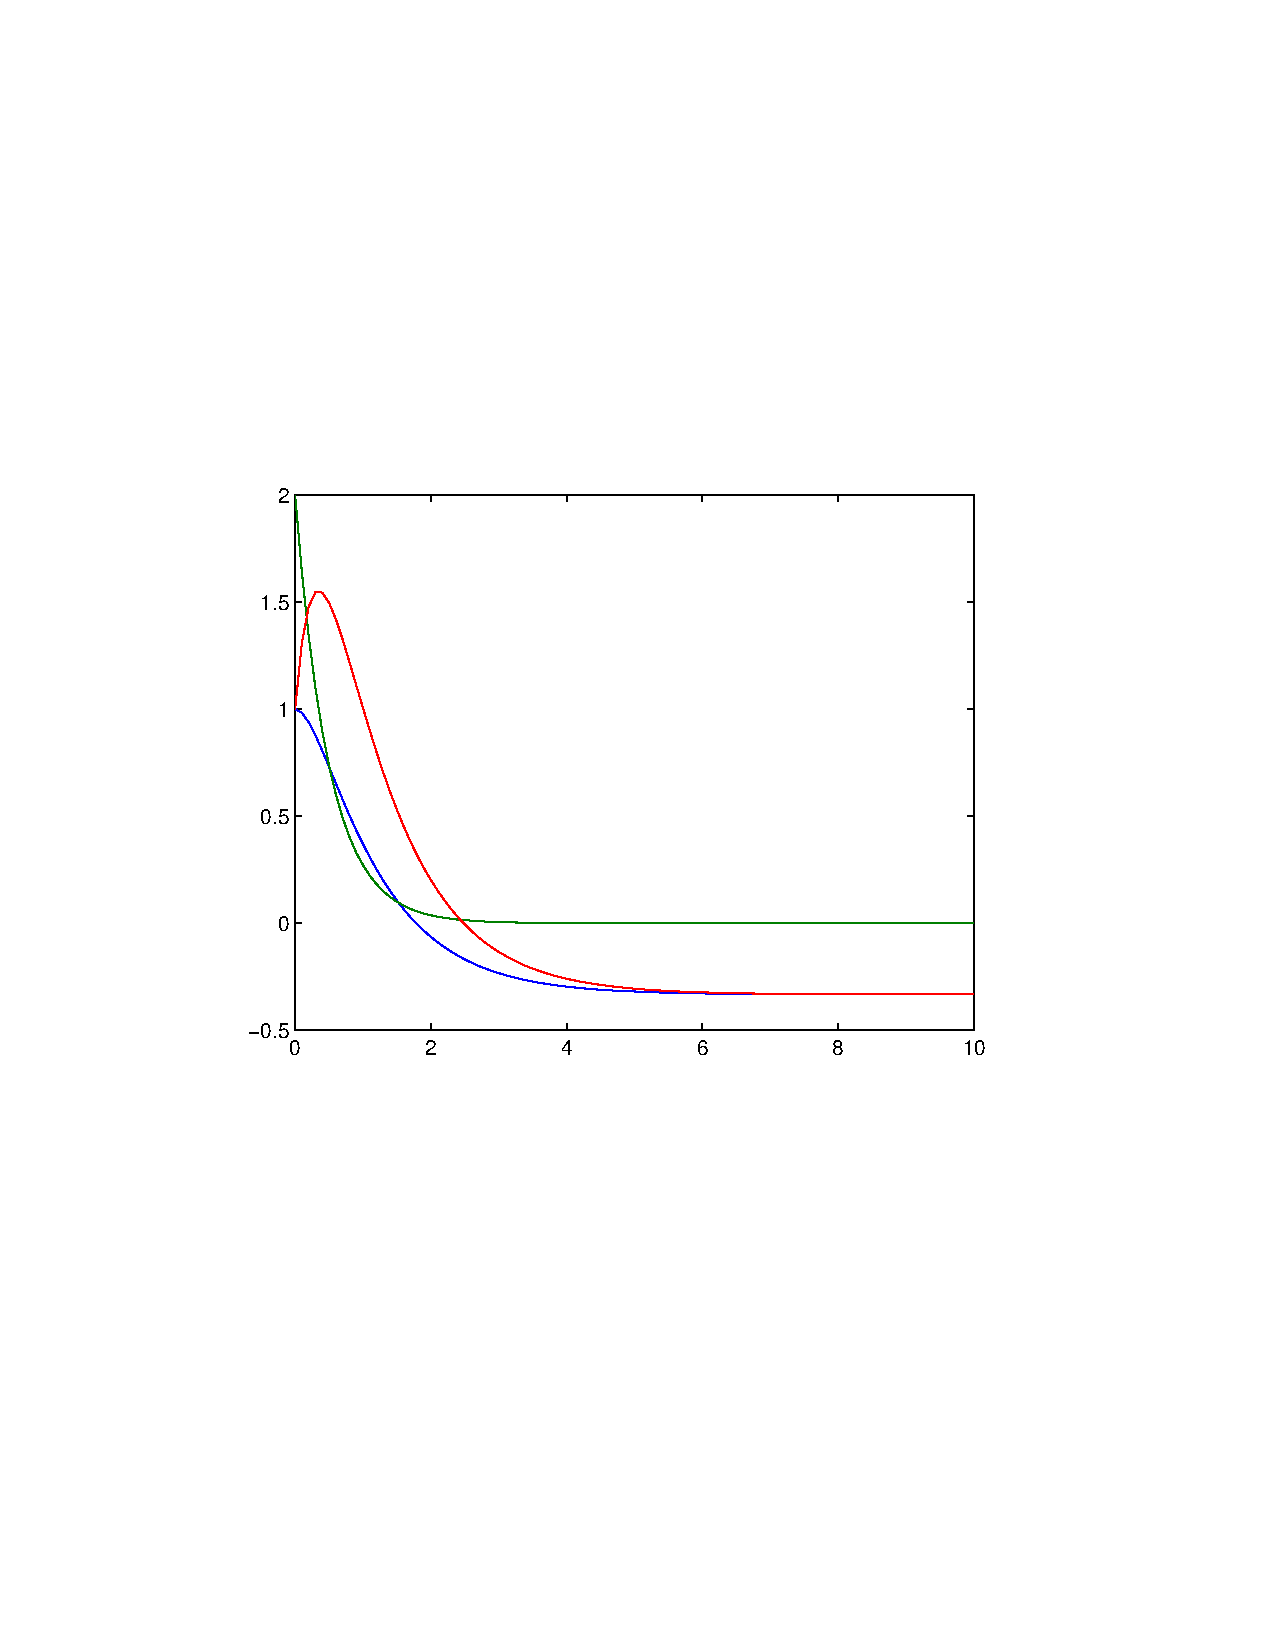
\includegraphics{num6} 
\caption{单位阶跃响应的系统状态轨迹图}
\end{figure*}
\end{document}


